\documentclass[12pt]{article}
\usepackage{/Users/kajal/Documents/statistics/resources/templates/HomeWorkTemplate}
\usepackage{circuitikz}
\usepackage[shortlabels]{enumitem}
\usepackage{hyperref}
\usepackage{tikz}
\usepackage{fontspec}
\usepackage{xepersian}
\usepackage{graphicx}
\usepackage{float}
\usepackage{changepage}

\usetikzlibrary{arrows,automata}
\usetikzlibrary{circuits.logic.US}
\settextfont{XB Niloofar}

\newcounter{problemcounter}
\newcounter{subproblemcounter}[problemcounter]
\newcounter{partcounter}[subproblemcounter]

\renewcommand{\thesubproblemcounter}{\alph{subproblemcounter})}
\renewcommand{\thepartcounter}{\roman{partcounter})}

\newcommand{\problem}[1]{
    \setcounter{subproblemcounter}{0}
    \stepcounter{problemcounter}
    \subsection*{پرسش \arabic{problemcounter} #1}
}

\newcommand{\subproblem}[1]{
    \setcounter{partcounter}{0}
    \stepcounter{subproblemcounter}
    \textbf{\harfi{subproblemcounter})}
}

\newcommand{\parte}[1]{
    \stepcounter{partcounter}
	\arabic{partcounter})
}



\begin{document}

\handout
{آمار و کاربرد ها}
{تمرین سری پنج}
{کژال باغستانی}
{۴۰۱۱۰۰۰۷۱}

\problem{}
\subproblem{}
 به سادگی مشخص است که این عبارت غلط است زیرا شخصی که از این رستوران سفارش داده است یا از قبل سفارش داده بوده
 که به وضوح راضی بوده و مشتری رستوران است و نظر او مثبت و در غیر این صورت این شخص از طرف شخصی دیگر
 که سلیقه های مشابهی دارند معرفی شده یا خودش در نگاه اول از رستوران راضی بوده که این رستوران را برای سفارش انتخاب کرده
 و در کل تعداد حالات کمی وجود دارد که شخص نظر منفی داشته باشد و این نمونه گیری به وضوح اریب است.
\newline
\subproblem{} 
این نمونه گیری نیز به دلایل مختلفی که چند نمونه را ذکر خواهم کرد اریب است. یکی اینکه ریاضی دو درسی پایه و اجباری است.
یکی دیگر اینکه درس فلسفه ریاضی فقط مربوط به دانشکده ریاضی و همجین درس اختیاری است در صورتی که 
ریاضی دو مربوط به کل دانشگاه و اجباری است.
یکی دیگر از دلایل این است که برای خیلی از دانشجویان نمره خوب را به سادگی گرفتن ملاک است ولی دکتر شهشهانی استادی
سخت گیر است.
\problem{}
\subproblem{}
از لحاظ مفهومی چولگی به معنای میزان دوری داده های پرت است یا به عبارتی علامت آن نشان دهنده راست یا چپ بودن داده های دور تر از میانگین یا مد است.

\subproblem{}
\begin{figure}[H]
	\centering
	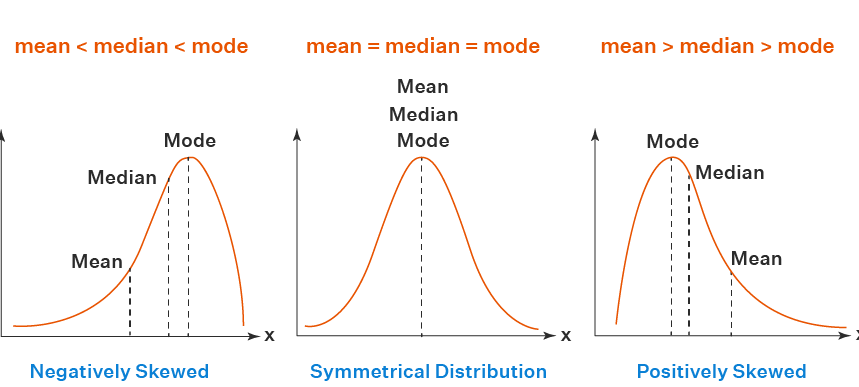
\includegraphics[width=0.5\textwidth]{/Users/kajal/Documents/statistics/resources/hw1/skewness.png}
\end{figure}
شکل بالا به وضوح به ما نشان میدهد که ترتیب میانگین و میانه و مد در چولگی به چپ و راست و توزیع متقارن به چه صورت است.
\\
\subproblem{}
برابر بودن ضریب اول و دوم پیرسن به ما رابطه زیر را می دهند:
\[
\frac{\bar{x} - M}{s} = \frac{3(\bar{x} - m)}{s} = 0.32
\]
که با قرار دادن میانگین و انحراف معیار به ترتیب داریم:
\[
\frac{29.6 - M}{6.5} = 0.32
\]
که به ما می‌دهد:
\[ M = 29.6 - (0.32 \times 6.5) = 27.52 \text{ (مد)} \]
و برای معادله دوم:
\[
\frac{3(29.6 - m)}{6.5} = 0.32
\]
که به ما می‌دهد:
\[ 29.6 - m = 0.693 \]
بنابراین:
\[ m \approx 29.6 - 0.693 = 28.907 \approx 28.9 \]

\problem{}
\[
  E[X] = \int_{b}^{\infty}{xf(x)dx} = 
  \frac{e^{\frac{b}{a}}}{a}\int_{b}^{\infty}{xe^{-x}} =
  \frac{(1+b)}{a}e^{\frac{b}{a}-b}
\]

از طرفی چون تابع چگالی است داریم:\\
\[
  1 = \int_{b}^{\infty}{f(x)dx} = 
  \frac{e^{\frac{b}{a}}}{a}\int_{b}^{\infty}{e^{-x}} =
  \frac{1}{a}e^{\frac{b}{a}-b}
\]
قرار میدهیم :\\
\[
    \bar{X} = \sum_{i = 0}^{n}{\frac{X_i}{n}}    
\]

 از طرفی دیگر داریم با روش گشتاور:\\
 \[
    \frac{(1+b)}{a}e^{\frac{b}{a}-b}  = \bar{X}
 \]

 می دانیم $\frac{1}{a}e^{\frac{b}{a}-b} = 1$
 پس در رابطه های بالا بجای این عبارت $1$ را قرار میدهیم داریم:\\
 \[
    1+b = \bar{X} \quad => \quad b = \bar{X} - 1
 \]
حالا باید $a$ را برحسب $b$ حل کنیم به صورتی که 
$\frac{1}{a}e^{\frac{b}{a}-b} = 1$
را حل کنیم که $a = 1$
در این معادله جواب میدهد و از آنجایی که تابع چگالی بر حسب a است و یکتاست
پس همین جواب کافیست و روش گشتاوری به ما برآورد گر های زیر را میدهد:\\
\[
    a = 1 \quad b = \bar{X} - 1
\]
توجه کنید که این معادله بر حسب $b = \bar{X} - 1$
 ممکن است جواب های دیگری نیز داشته باشد برای $a$
 اما یکی از جواب ها حتما همیشه $1$
 است که از داده مستقل است همچنین جواب دیگر را میتوان بر حسب داده به صورت ضمنی محاسبه کرد.
 که رابطه ضمنی ما هست:\\
 \[
    b = \bar{X} - 1 =\frac{a}{1-a}\log^{a}
 \]









%  \[
%     \frac{(b^2)}{a}e^{\frac{b}{a}-b} 
%     +2\frac{(b+1)}{a}e^{\frac{b}{a}-b} 
%     = \sigma^2
%  \]
%  \[
%     \frac{(b^2+2b+2)}{\sigma^2}e^{\frac{b}{a}-b} = a
%  \]
% %  \[
% %     \frac{(b^2)}{a}e^{\frac{b}{a}-b} = \sigma^2 - 2\bar{X}
% %  \]

%  \[
%     \frac{(b^2)}{a}e^{\frac{b}{a}-b} = \sigma^2 - 2\bar{X}
%  \]

%  \[
%     \frac{({\log^{a}\frac{a}{1-a}})^2}{a}e^{\frac{\log^{a}\frac{a}{1-a}}{a}-\log^{a}\frac{a}{1-a}} = \sigma^2 - 2\bar{X}
%  \]



% \[
%     \frac{E[X]}{E[X^2]} =  \frac{\bar{X}}{\sigma^2} = \frac{1+b}{b^2+2b+2}
% \]
% \[
%   E[X^2] = \int_{b}^{\infty}{x^2f(x)dx} = 
%   \frac{e^{\frac{b}{a}}}{a}\int_{b}^{\infty}{x^2e^{-x}} =
%   \frac{(b^2+2b+2)}{a}e^{\frac{b}{a}-b}
% \]

% و
% \[
%     \sigma^2 = \sum_{i = 0}^{n}{\frac{{X_i}^2}{n}}    
% \]
% \[
    % \frac{(b^2+2b+2)}{a}e^{\frac{b}{a}-b} = \sigma^2
%  \]
\problem{}
تفکر تفکر
\problem{}
اگر فرض کنیم $p$
را با $\hat{p}$
بر آورد کنیم احتمال این رخداد برابر است با:\\
\[
    f(\hat{p}) = \hat{p}^k (1-\hat{p})^{n-k}
\]
حالا طبق این روش برای بدست آوردن ماکسیمم تابع بالا
 باید از تابع بالا نسبت به $\hat{p}$
مشتق بگیریم داریم:\\
\[
    f^{\prime}(\hat{p}) =  k\hat{p}^{k-1}(1-\hat{p})^{n-k} - (n-k)\hat{p}^k(1-\hat{p})^{n-k-1}
\]
اگر این عبارت را برابر صفر قرار دهیم داریم:\\
\[
    k(1-\hat{p}) =\hat{p}(n-k)
\]
که این روش پیشنهاد میدهد قرار دهیم$\hat{p} = \frac{k}{n} \quad$.\\\\
(به این نکته توجه کنید که این تابع در نقاط دو سر بازه
ماکسیمم نمیشود $f(0) = f(1) = 0$)
\problem{}


\subproblem{}
در این حالت هر استراتژی ما در نهایت به یک دنباله 
از شماره و خال کارت ها تقسیم میشود که وقتی هیچ اطلاعاتی ا
ز کارت ها نداریم، دنباله ما صرفا یک جایگشت رندوم از کل کارت ها است. پس برای محاسبه $E[N]$ می توانیم متغیر تصادفی $X_i$ را تعریف کنیم که بر
نولی درست بودن کارت $i$ ام را نشان می‌دهد.  
\\
\[ E[N] = \sum_{i=1}^{52}E[X_i] = 52 \times \frac{1}{52} = 1 \]

\subproblem{}
در این قسمت، در هر استراتژی، نهایت اطلاعات ما در مرحله $i$ ام این است که کارت های ۱ تا $i-1$ چه بوده اند که می‌توانیم از گفتن آنها برای کار
ت $i$ ام صرف نظر کنیم. پس دوباره مثل قسمت قبل می‌توانیم $X_i$ ها را تعریف کنیم و 
این بار داریم:
\[ E[N] = \sum_{i=1}^{n}E[X_i] = \sum_{i=1}^{n} \frac{1}{n - i + 1} \approx \ln{n} \]

\problem{}
برای حل این سوال و تخمین $\frac{\sigma_1}{\sigma_2}$
از توزیع fraction استفاده میکنیم.\\
داریم :\\
\[ (\frac{S_2 .\sigma_1}{S_1.\sigma_2})^2 \sim F(m-1,n-1) \]
در نتیجه:\\
\[ P[\frac{\sigma_1 ^2}{\sigma_2 ^2} \leq \frac{S_1 ^2}{S_2 ^2}a] = F(a)\]
\\
که $n = 247.3\times 40 = 9892 $ و $m = 254.1 \times 30 = 7623$
پس با کمک اینترنت $a = 1.036$.\\
که :\\
\[ F(a) = 0.95 \]
\[ P[\frac{\sigma_1 ^2}{\sigma_2 ^2} \leq \frac{231.04}{349.69}1.036] =
P[\frac{\sigma_1 ^2}{\sigma_2 ^2} \leq 0.684] = 0.95\]



\end{document}

